%!TEX root = ../novoIndex.tex

\subsection{Abordagem 1}

A primeira abordagem de treinamento das CNNs constitiu na utilização das imagens da base de dados sem pré-processamento. Duas funções de ativação distintas: relu (introduz não linearidade),lrelu (usado na literatura ...)
Não há utilização de pesos previamente calculados.

- Normalização das imagens
- 1 técnica de data augmentation: horizontal flip

(\ldots)
% Explicação da le net, gráficos da le net

% Explicação da alexnet, gráficos da alexnet


%% Sumário
%% Tabela
%  Rede | Função de ativação | Parâmetros | Tempo de treinamento | RMSE obtido | MAE obtido


Considerando a abordagem descrita na solução proposta, os resultados preliminares da execução das CNNs aplicadas ao problema de estimação de idade a partir de uma imagem de face são apresentados a seguir.

Conforme mencionado na Seção \ref{subsec:modelos}, os primeiros treinamentos e testes compreenderam as arquiteturas canônicas LeNet e AlexNet com função de ativação \emph{ReLU} na camada de saída, tendo como entrada as imagens do conjunto de dados sem normalização e equalização. Obedecendo ao método de validação cruzada \emph{holdout} previamente mencionado, os resultados da etapa de teste foram obtidos, detalhados na Tabela \ref{tab:results_relu}.

\begin{table}[!ht]
     \caption{Resultados preliminares do treino e teste dos modelos propostos utilizando \emph{ReLU} na camada de saída.}
     \label{tab:results_relu}
     \centering
     \begin{tabular}{l l l}
          \toprule
          Modelo & Épocas &RMSE \\
          \midrule
          LeNet & $95$ & $41.08$ \\
          AlexNet & $55$ & $41.96$\\
          \bottomrule
     \end{tabular}
\end{table}

Ao observar as previsões realizadas para exemplos individuais, percebeu-se uma tendência destas redes após treinamento em preverem valores baixos, indicando possivelmente \emph{underfitting} em virtude do \emph{ReLU dying problem} \cite{djork2015elus, dabal2018elus}. Como alternativa, estes autores sugerem  utilizar variantes da \emph{ReLU} que não exibam saídas nulas, diferentes estratégias de inicialização e regularização de pesos e \emph{batches}, entre outras. Como exposto na Seção \ref{subsec:modelos}, adotou-se a \emph{Leaky ReLU} como função de ativação da camada de saída. Os resultados deste treinamento estão expostos na Tabela \ref{tab:results_leaky}.

\begin{table}[!ht]
     \caption{Resultados preliminares do treino e teste dos modelos propostos utilizando \emph{Leaky ReLU} na camada de saída.}
     \label{tab:results_leaky}
     \centering
     \begin{tabular}{l l l}
          \toprule
          Modelo & Épocas & RMSE \\
          \midrule
          LeNet & $12$ & $41.55$ \\
          AlexNet & $6$ & $14.38$\\
          \bottomrule
     \end{tabular}
\end{table}

Observa-se que houve uma resposta positiva da AlexNet que melhorou a qualidade das previsões para o problema considerado. Porém, observa-se uma tendência desta rede em prever valores médios, o que ainda enseja melhorias. Assim, ainda é necessário investigar outros parâmetros e modelos para o problema em questão.


\begin{figure}[hb!]
	\caption{Redes neurais biológicas.}
	\begin{subfigure}[hb]{0.5\linewidth}
		\caption{Treinamento Alexnet LRelU com imagens normalizadas e equalizadas}
		\label{fig:histalexlrelunorm}
    \centering
		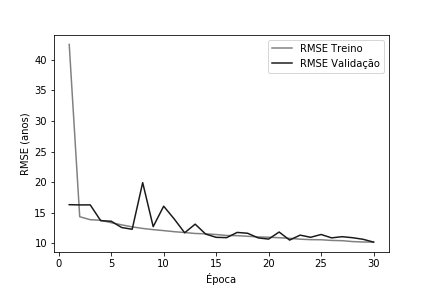
\includegraphics[width=\linewidth]{img/graficos-fase2/fig-history-alexnet-lrelu-data-augmentation-22.png}
	\end{subfigure}
	\begin{subfigure}[hb]{0.5\linewidth}
		\caption{Treinamento Alexnet ReLU com imagens normalizadas e equalizadas}
		\label{fig:redeneuralbiologica}
		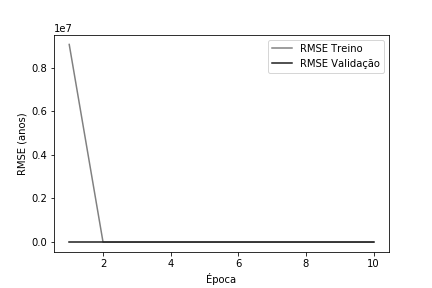
\includegraphics[width=\linewidth]{img/graficos-fase2/fig-history-alexnet-relu-data-augmentation-21.png}
	\end{subfigure}\\
  \begin{subfigure}[hb]{0.5\linewidth}
    \caption{Treinamento LeNet ReLU com imagens normalizadas e equalizadas}
    \label{fig:redeneuralbiologica}
    \includegraphics[width=\linewidth]{img/graficos-fase2/fig-history-lenet-relu-data-augmentation-21.png}%
  \end{subfigure}%
  % \begin{subfigure}[hb]{0.5\linewidth}
  %   \caption{Treinamento LeNet RelU com imagens normalizadas e equalizadas}
  %   \label{fig:redeneuralbiologica}
  %   \includegraphics[width=\linewidth]{img/grafico-fase2/fig-history-lenet-relu-data-augmentation-21}
  % \end{subfigure}%
\end{figure}


\begin{figure}[hb!]
	\caption{Redes neurais biológicas.}
	\begin{subfigure}[hb]{0.5\linewidth}
		\caption{Reta-0 Alexnet LRelU com imagens normalizadas e equalizadas}
		\label{fig:histalexlrelunorm}
		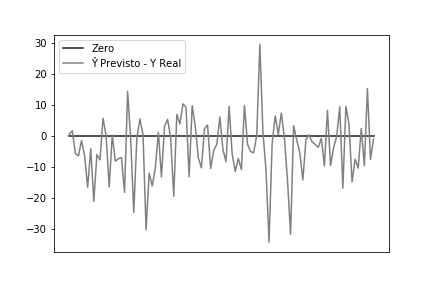
\includegraphics[width=\linewidth]{img/graficos-fase2/fig-reta-0-alexnet-lrelu-data-augmentation-22.png}
	\end{subfigure}%
	\begin{subfigure}[hb]{0.5\linewidth}
		\caption{Reta-0 Alexnet ReLU com imagens normalizadas e equalizadas}
		\label{fig:redeneuralbiologica}
		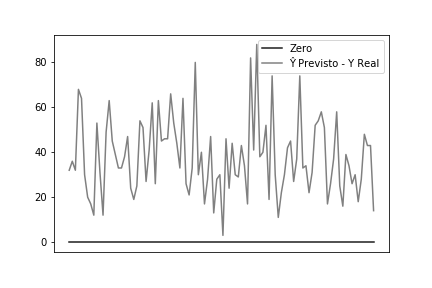
\includegraphics[width=\linewidth]{img/graficos-fase2/fig-reta-0-alexnet-relu-data-augmentation-21.png}
	\end{subfigure}%
  \begin{subfigure}[hb]{0.5\linewidth}
    \caption{Reta-0 LeNet ReLU com imagens normalizadas e equalizadas}
    \label{fig:redeneuralbiologica}
    \includegraphics[width=\linewidth]{img/graficos-fase2/fig-reta-0-lenet-relu-data-augmentation-21.png}%
  \end{subfigure}%
  % \begin{subfigure}[hb]{0.5\linewidth}
  %   \caption{Reta-0 LeNet RelU com imagens normalizadas e equalizadas}
  %   \label{fig:redeneuralbiologica}
  %  \includegraphics[width=\linewidth]{img/grafico-fase2/fig-reta-0-lenet-relu-data-augmentation-21}
  % \end{subfigure}%
\end{figure}

\begin{figure}[hb!]
	\caption{Redes neurais biológicas.}
	\begin{subfigure}[hb]{0.5\linewidth}
		\caption{Diferença de previsões Alexnet LRelU com imagens normalizadas e equalizadas}
		\label{fig:histalexlrelunorm}
		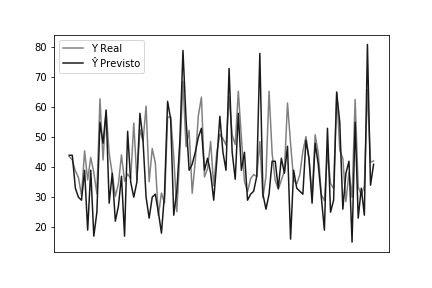
\includegraphics[width=\linewidth]{img/graficos-fase2/fig-reta-dif-alexnet-lrelu-data-augmentation-22.png}
	\end{subfigure}%
	\begin{subfigure}[hb]{0.5\linewidth}
		\caption{Diferença de previsões Alexnet ReLU com imagens normalizadas e equalizadas}
		\label{fig:redeneuralbiologica}
		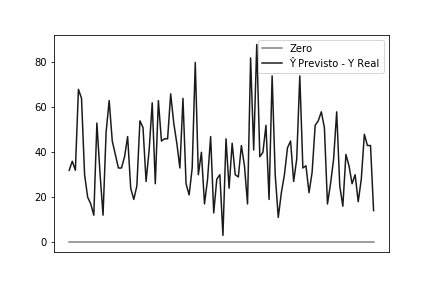
\includegraphics[width=\linewidth]{img/graficos-fase2/fig-reta-dif-alexnet-relu-data-augmentation-21.png}
	\end{subfigure}%
  \begin{subfigure}[hb]{0.5\linewidth}
    \caption{Diferença de previsões LeNet ReLU com imagens normalizadas e equalizadas}
    \label{fig:redeneuralbiologica}
    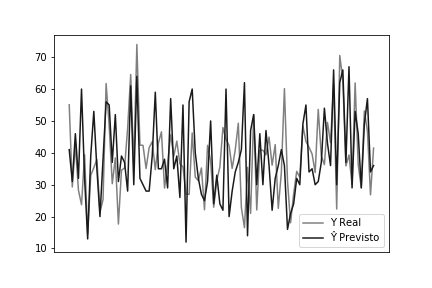
\includegraphics[width=\linewidth]{img/graficos-fase2/fig-reta-dif-lenet-relu-data-augmentation-21.png}%
  \end{subfigure}%
  % \begin{subfigure}[hb]{0.5\linewidth}
  %   \caption{Diferença de previsões LeNet RelU com imagens normalizadas e equalizadas}
  %   \label{fig:redeneuralbiologica}
  %   \includegraphics[width=\linewidth]{img/grafico-fase2/fig-reta-dif-lenet-relu-data-agmentation-21}
  % \end{subfigure}%
\end{figure}

\subsection{Abordagem 2}

- Mesmas redes
- Normalização das imagens, equalização por histograma -> o que é
- data augmentation ->  mais técnicas de data augmentation

\subsection{Abordagem 3}

Outras arquiteturas
VGG
com transfer learning
1. Retirar última camada (softmax) e adicionar leaky relu
2. Retirar duas últimas camadas (dense e softmax) e adicionar leaky relu
